\documentclass{beamer}
%\documentclass[xcolor=dvipsnames]{beamer}
\usepackage[spanish]{babel}
\usepackage[utf8]{inputenc}
\usepackage{graphicx}
\usepackage{csquotes}
\usepackage{algorithm,algorithmic}
\usepackage[]{algorithm2e}

\newcommand{\beamer}{\textsc{beamer}}
\newtheorem{definicion}{Definición}
\newtheorem{ejemplo}{Ejemplo}

%%%%%%%%%%%%%%%%%%%%%%%%%%%%%%%%%%%%%%%%%%%%%%%%%%%%%%%%%%%%%%%%%%%%%%%%%%%%%%%
\title[genetics.js]{
    genetics.js \\
    Framework web de computación evolutiva
}
\author[Cristian Abrante]{Cristian Manuel Abrante Dorta}
\institute[ULL]{Universidad de La Laguna}
\date[21-06-2019]{\today}
%%%%%%%%%%%%%%%%%%%%%%%%%%%%%%%%%%%%%%%%%%%%%%%%%%%%%%%%%%%%%%%%%%%%%%%%%%%%%%%

\usetheme{Madrid}
%\usetheme{Warsaw}

%%%%%%%%%%%%%%%%%%%%%%%%%%%%%%%%%%%%%%%%%%%%%%%%%%%%%%%%%%%%%%%%%%%%%%%%%%%%%%%
\definecolor{pantone254}{RGB}{87,6,140}
\definecolor{pantone3015}{RGB}{0,88,147}
\definecolor{pantone432}{RGB}{56,61,66}
\setbeamercolor*{palette primary}{use=structure,fg=white,bg=pantone254}
\setbeamercolor*{palette secondary}{use=structure,fg=white,bg=pantone3015}
\setbeamercolor*{palette tertiary}{use=structure,fg=white,bg=pantone432}
\setbeamercolor*{palette sidebar primary}{use=structure,fg=pantone254}
\setbeamercolor*{palette sidebar tertiary}{use=structure,fg=pantone3015}
\setbeamercolor*{block title}{bg=pantone3015,fg=white}
\setbeamercolor*{alerted text}{fg=pantone432}
\setbeamercolor*{item projected}{fg=pantone254}
\setbeamercolor*{section in toc shaded}{use=structure,fg=structure.fg}
\setbeamercolor*{section in toc}{fg=pantone3015}
\setbeamercolor*{subsection in toc shaded}{fg=pantone3015}
\setbeamercolor*{subsection in toc}{fg=pantone432}

%%%%%%%%%%%%%%%%%%%%%%%%%%%%%%%%%%%%%%%%%%%%%%%%%%%%%%%%%%%%%%%%%%%%%%%%%%%%%%%
\begin{document}
  
%++++++++++++++++++++++++++++++++++++++++++++++++++++++++++++++++++++++++++++++  
\begin{frame}

  
\includegraphics[width=0.45\textwidth]{pres/img/etsit-logo.png}
  \hspace*{2cm}
  
\includegraphics[width=0.35\textwidth]{pres/img/geneticsjs-logo.png}
  \titlepage

  \begin{scriptsize}
    \begin{center}
     Escuela Superior de Ingeniería y Tecnología \\
     Universidad de La Laguna
    \end{center}
  \end{scriptsize}

\end{frame}
%++++++++++++++++++++++++++++++++++++++++++++++++++++++++++++++++++++++++++++++  

%++++++++++++++++++++++++++++++++++++++++++++++++++++++++++++++++++++++++++++++  
\begin{frame}
  \frametitle{Índice}  
  \tableofcontents
\end{frame}
%++++++++++++++++++++++++++++++++++++++++++++++++++++++++++++++++++++++++++++++  

\section{Introducción}

%++++++++++++++++++++++++++++++++++++++++++++++++++++++++++++++++++++++++++++++  

\subsection{$\mathcal{P}$ vs $\mathcal{NP}$}

%++++++++++++++++++++++++++++++++++++++++++++++++++++++++++++++++++++++++++++++  
\begin{frame}
\frametitle{$\mathcal{P}$ vs $\mathcal{NP}$}

En primer lugar, veremos una clasificación de los problemas en función de su complejidad.

\begin{figure}
    \centering
    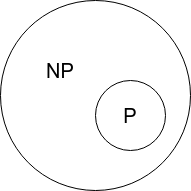
\includegraphics[scale=0.5]{pres/img/introduccion/p-np.png}
    \caption{Representación de las clases de problemas $\mathcal{P}$ y $\mathcal{NP}$}
    \label{fig:p-np}
\end{figure}

\begin{itemize}
    \item \textbf{Clase $\mathcal{P}$}: Se puede encontrar una solución en \textbf{tiempo polinomial}.
    \item \textbf{Clase $\mathcal{NP}$}: Se puede verificar una solución en \textbf{tiempo polinomial}.
\end{itemize}

\end{frame}
%++++++++++++++++++++++++++++++++++++++++++++++++++++++++++++++++++++++++++++++  

\subsection{Optimización combinatoria}

%++++++++++++++++++++++++++++++++++++++++++++++++++++++++++++++++++++++++++++++  
\begin{frame}
\frametitle{Optimización combinatoria}

Dentro de la clase $\mathcal{NP}$, existen una gran cantidad de problemas de \textbf{optimización combinatoria}. \\

\begin{block}{Optimización combnatoria}
 En este tipo de problemas, se trata de optimizar una función objetivo, que depende de una serie de variables \textbf{discretas}, sujetas a un conjunto de restricciones.
\end{block}
\\
Algunos ejemplos de este tipo de problemas:

\begin{itemize}
    \item Problema del viajante de comercio (TSP).
    \item Problema de rutas y capacidades de vehículos (VRP).
\end{itemize}
\end{frame}
%++++++++++++++++++++++++++++++++++++++++++++++++++++++++++++++++++++++++++++++

%++++++++++++++++++++++++++++++++++++++++++++++++++++++++++++++++++++++++++++++
\begin{frame}
\frametitle{Optimización combinatoria}

Formalmente, un problema ($P$) de optimización combinatoria se puede definir como una tupla:

\begin{center}
    $P = (S, f, \Omega)$
\end{center}

Donde:

\begin{itemize}
    \item \textbf{Espacio de soluciones} ($S$): Es el conjunto finito y numerable de todas las posibles soluciones al problema.
    \item \textbf{Función objetivo} ($f$): Para cada solución de $S$, devuelve su valor de bondad.
    \begin{center}
        \begin{math}
            f: S \rightarrow \mathbb{R}
        \end{math}
    \end{center}
    \item \textbf{Conjunto de restricciones} ($\Omega$): Conjunto de restricciones que debe satisfacer una solución de s ($s \in S$), para ser válida.
\end{itemize}

\end{frame}
%++++++++++++++++++++++++++++++++++++++++++++++++++++++++++++++++++++++++++++++

%++++++++++++++++++++++++++++++++++++++++++++++++++++++++++++++++++++++++++++++
\begin{frame}
\frametitle{Optimización combinatoria}

El concepto de \textbf{óptimo global} ($s^*$) es la solución para la cual la función objetivo tiene una evaluación más alta:

\begin{center}
    $\forall s \in S, \quad f(s^*) \geq f(s)$ 
\end{center}

Para encontrar esta solución, existen varias opciones:

\begin{itemize}
    \item Enumerar todas las soluciones de $S$. Esto suele ser \textbf{inviable} debido al gran tamaño de este conjunto.
    \item Utilizar una \textbf{exploración inteligente} del espacio de soluciones. Utilizando por ejemplo, \textbf{metaheurísticas}.
\end{itemize}

\end{frame}
%++++++++++++++++++++++++++++++++++++++++++++++++++++++++++++++++++++++++++++++

\subsection{Metaheurísticas}

%++++++++++++++++++++++++++++++++++++++++++++++++++++++++++++++++++++++++++++++
\begin{frame}
\frametitle{Metaheurísticas}

\begin{block}{Metaheurísticas}
 Las metaheurísticas se centran en encontrar soluciones a problemas de optimización aplicando una búsqueda en el espacio de soluciones ($S$), cuando no se tiene información específica del problema.
\end{block}

\bigskip

Existen muchas técnicas metaheurísticas, que se pueden clasificar según diferentes criterios, sin embargo en este trabajo nos centraremos en la \textbf{computación evolutiva}.

\end{frame}
%++++++++++++++++++++++++++++++++++++++++++++++++++++++++++++++++++++++++++++++  

\section{Computación evolutiva}

%++++++++++++++++++++++++++++++++++++++++++++++++++++++++++++++++++++++++++++++  

\subsection{Definición}

%++++++++++++++++++++++++++++++++++++++++++++++++++++++++++++++++++++++++++++++  
\begin{frame}
\frametitle{Computación evolutiva}

\begin{exampleblock}{}
  {\large ``La gran ventaja de la evolución es la gran cantidad de especies diferentes que ha creado, cada una adaptada a su medio''}
  \vskip5mm
  \hspace*\fill{\small--- A.E. Eiben y J.E. Smith}
\end{exampleblock}

\begin{block}{Computación evolutiva}
 La \textbf{computación evolutiva} es una técnica metaheurística, bio-inpirada y basada en población. Utilizada para resolver diversos problemas complejos, y especialmente útil a la hora de resolver problemas de \textbf{optimización combinatoria}.
\end{block}

\end{frame}
%++++++++++++++++++++++++++++++++++++++++++++++++++++++++++++++++++++++++++++++  

\subsection{Historia}

%++++++++++++++++++++++++++++++++++++++++++++++++++++++++++++++++++++++++++++++  
\begin{frame}
\frametitle{Historia}

\begin{columns}
\column{0.5\textwidth}
La inspiración principal de la computación evolutiva es la \textbf{Teoría de la evolución de Darwin}. En la cual se exponen conceptos clave como la \textbf{selección natural} o la \textbf{supervivencia de los individuos más adaptados}.

\column{0.5\textwidth}
\begin{figure}
    \centering
    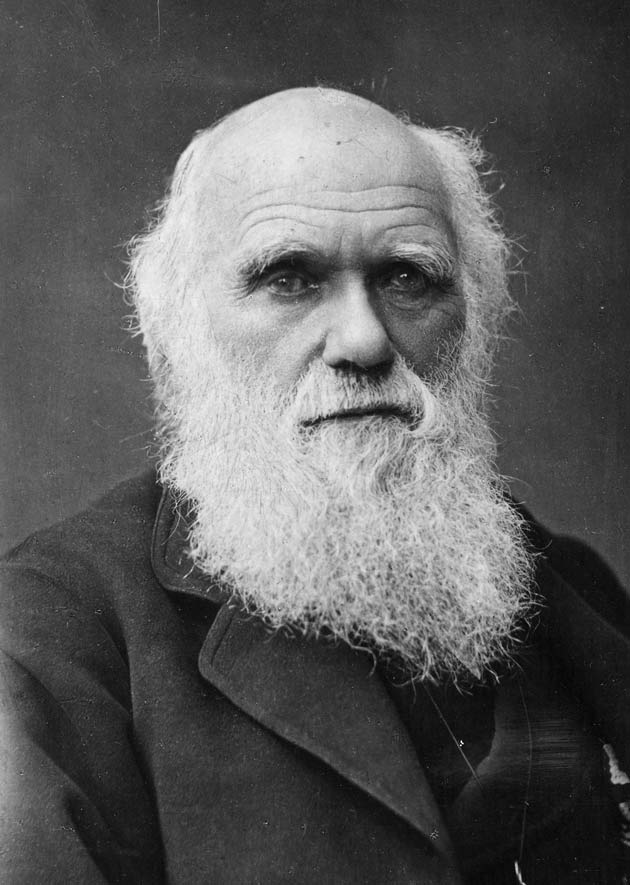
\includegraphics[scale=0.15]{pres/img/darwin.jpg}
    \caption{Charles Darwin}
    \label{fig:darwin}
\end{figure}
\end{columns}

\end{frame}
%++++++++++++++++++++++++++++++++++++++++++++++++++++++++++++++++++++++++++++++

%++++++++++++++++++++++++++++++++++++++++++++++++++++++++++++++++++++++++++++++  
\begin{frame}
\frametitle{Historia}

El desarrollo de la computación evolutiva se produce a partir de los \textbf{años sesenta}:

\begin{description}
    \item[1962] Bremermann ejecuta el primer experimento sobre \textbf{Optimización mediante evolución y recombinación}.
    \item[1965] Fogel, Owen y Walsh introducen el término de \textbf{Programación evolutiva}.
    \item[1973] Holland desarrolla los \textit{algoritmos genéticos}.
    \item[1973] Rechenberg y Schwefel crean las \textbf{estrategias evolutivas}.
    \item[1990] Se unifican todos los términos, definiendo el término \textbf{computación evolutiva}
\end{description}

\end{frame}
%++++++++++++++++++++++++++++++++++++++++++++++++++++++++++++++++++++++++++++++  

\subsection{Estructura}

%++++++++++++++++++++++++++++++++++++++++++++++++++++++++++++++++++++++++++++++  
\begin{frame}
\frametitle{Estructura}

La estructura de un algoritmo evolutivo es la siguiente:

\begin{algorithm}[H]
 INICIALIZAR la población con $n$ individuos aleatorios;\\
 EVALUACIÓN de la población mediante la función de puntuación (\textit{fitness});
 
 \While{CONDICIÓN DE PARADA no sea satisfecha}{
  SELECCIÓN de padres; \\
  RECOMBINACIÓN de pares de padres; \\
  MUTACIÓN de la descendencia; \\
  EVALUACIÓN de la descendencia; \\
  SELECCIÓN de supervivientes para la siguiente generación;
 }
 \caption{Esquema básico de un algoritmo evolutivo}
\end{algorithm}

\end{frame}
%++++++++++++++++++++++++++++++++++++++++++++++++++++++++++++++++++++++++++++++  

%++++++++++++++++++++++++++++++++++++++++++++++++++++++++++++++++++++++++++++++ 
\begin{frame}
\frametitle{Estructura}

Los algoritmos evolutivos permiten realizar una exploración inteligente del espacio de soluciones ($S$) del problema gracias a:

\bigskip

\begin{itemize}
    \item \textbf{Variación}: Las fases de mutación y recombinación garantizan la diversidad en las soluciones.
    \item \textbf{Intensificación}: Las fases de selección de padres y descendencia, garantizan que se evaluen las mejores soluciones.
\end{itemize}

\end{frame}
%++++++++++++++++++++++++++++++++++++++++++++++++++++++++++++++++++++++++++++++

\section{Objetivos}

%++++++++++++++++++++++++++++++++++++++++++++++++++++++++++++++++++++++++++++++

\subsection{Bibliotecas de algoritmos evolutivos}

%++++++++++++++++++++++++++++++++++++++++++++++++++++++++++++++++++++++++++++++ 
\begin{frame}
\frametitle{Bibliotecas de algoritmos evolutivos}

Existen numerosas bibliotecas de algoritmos evolutivos, que contienen una implementación de los métodos más comunes existentes en cada fase. \\

\bigskip

\begin{itemize}
    \item \textbf{Desarrolladas en Java}: Opt4J, Optimization Algorithm Toolkit, JMetal, ...
    \item \textbf{Desarrolladas en C++}: ParadisEO, METCO,..
\end{itemize}

\bigskip

Se ha identificado la carencia de un \textit{framework} de este propósito, pero \textbf{orientado a aplicaciones web}.

\end{frame}
%++++++++++++++++++++++++++++++++++++++++++++++++++++++++++++++++++++++++++++++

\subsection{Objetivos}

%++++++++++++++++++++++++++++++++++++++++++++++++++++++++++++++++++++++++++++++ 
\begin{frame}
\frametitle{Objetivos}

\begin{block}{Desarrollo}
 El objetivo de este proyecto es el desarrollo de un \textit{framework} que contenga los principales métodos que cubran todas las fases de un algoritmo evolutivo.
\end{block}

\bigskip

Además debe cumplir los siguientes criterios:

\begin{itemize}
    \item Garantizar la compatibilidad con aplicaciones web.
    \item Estar implementado en un lenguaje de programación moderno y soportado por la comunidad.
    \item Utilizar herramientas que garanticen la continuidad del proyecto.
    \item Contar con una buena documentación.
    \item Garantizar que pueda ser extensible.
\end{itemize}

\end{frame}
%++++++++++++++++++++++++++++++++++++++++++++++++++++++++++++++++++++++++++++++

\subsection{Roadmap}

%++++++++++++++++++++++++++++++++++++++++++++++++++++++++++++++++++++++++++++++ 
\begin{frame}
\frametitle{Objetivos}

Para cumplir estos criterios y objetivos se ha elaborado un \textbf{Roadmap} basado en \textbf{semantic versioning}:

\bigskip

\begin{itemize}
    \item \texttt{0.1.0}: Implementación de la codificación de soluciones mediante \textbf{individuos}.
    \item \texttt{0.2.0}: Implementación de los operadores de mutación.
    \item \texttt{0.3.0}: Impelementación de los operadores de cruce.
    \item \texttt{0.4.0}: Implementación de los operadores de selección de padres. 
    \item \texttt{0.5.0}: Implementación de los operadores de selección de supervivientes.
    \item \texttt{0.6.0}: Implementación de las clases gestoras de la población de individuos.
\end{itemize}

\end{frame}
%++++++++++++++++++++++++++++++++++++++++++++++++++++++++++++++++++++++++++++++

%++++++++++++++++++++++++++++++++++++++++++++++++++++++++++++++++++++++++++++++
\begin{frame}
  \frametitle{Bibliografía}

  \begin{thebibliography}{10}

    \beamertemplatebookbibitems
    \bibitem[URL: CTAN]{latex} 
    CTAN. {\small $http://www.ctan.org/$}

    \beamertemplatebookbibitems
    \bibitem[Tantau, 2005]{beamer} 
    Tantau, Till. 
    \emph{User's Guide to the \beamer{} Class, Version 3.06, 2005} 
    {\small $http://ctang.tug.org/tex-archive/macros/latex/contrib/beamer$}


  \end{thebibliography}
\end{frame}
%++++++++++++++++++++++++++++++++++++++++++++++++++++++++++++++++++++++++++++++  

\end{document}
